\documentclass[border=4pt]{standalone}
\usepackage[T1]{fontenc}
\usepackage{tikz}
\usetikzlibrary{
  positioning, arrows.meta, calc, fit, backgrounds,
  shapes.geometric, decorations.pathreplacing
}
\usepackage{amsmath,amssymb}

\definecolor{datablue}{HTML}{4A90D9}
\definecolor{gepagreen}{HTML}{6AB04C}
\definecolor{evalorange}{HTML}{E67E22}
\definecolor{qwkpurple}{HTML}{9B59B6}
\definecolor{trustred}{HTML}{D9534F}
\definecolor{pricegray}{HTML}{95A5A6}
\definecolor{bgblue}{HTML}{EBF5FB}
\definecolor{bggreen}{HTML}{EEF8EA}
\definecolor{bgorange}{HTML}{FEF3E8}
\definecolor{bggray}{HTML}{F4F6F7}

\tikzset{
  B/.style={draw, rounded corners=2pt, minimum height=7mm,
    minimum width=20mm, align=center, font=\scriptsize\sffamily, line width=0.5pt},
  S/.style={draw, rounded corners=1.5pt, minimum height=6mm,
    minimum width=18mm, align=center, font=\tiny\sffamily, line width=0.4pt},
  H/.style={draw, rounded corners=2pt, minimum height=8mm,
    minimum width=22mm, align=center, font=\scriptsize\sffamily\bfseries,
    line width=0.6pt},
  D/.style={draw=black!50, fill=bggray, rounded corners=1.5pt,
    minimum height=6mm, align=center, font=\tiny\sffamily},
  R/.style={draw=trustred, fill=trustred!8, rounded corners=2pt,
    minimum height=7mm, minimum width=20mm, align=center,
    font=\scriptsize\sffamily\bfseries, line width=0.6pt},
  a/.style={-{Stealth[length=1.8mm]}, line width=0.45pt},
  da/.style={-{Stealth[length=1.8mm]}, line width=0.45pt, dashed},
  d/.style={font=\fontsize{5}{6}\selectfont\sffamily, text=black!55},
}

\begin{document}
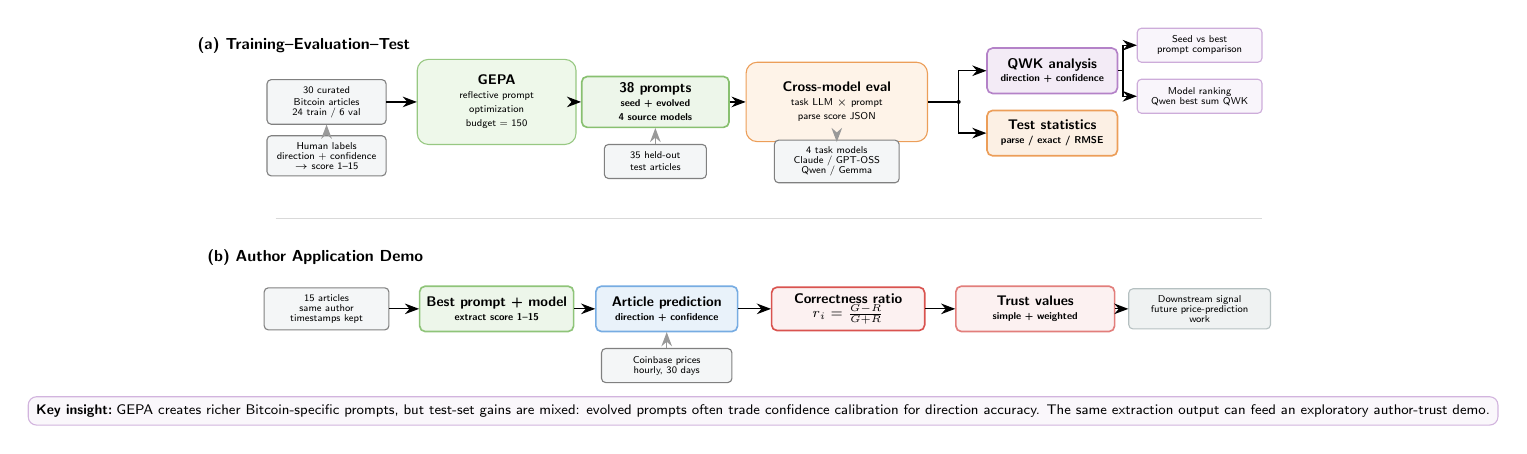
\begin{tikzpicture}[scale=0.72, transform shape]

% ═══════════════════════════════════════════════════════════════
% (a) TRAINING / EVALUATION / TEST — main research workflow
% ═══════════════════════════════════════════════════════════════
\node[font=\footnotesize\sffamily\bfseries] at (-1.2, 1.0)
  {(a) Training--Evaluation--Test};

% Data and labels
\node[D, minimum width=21mm] at (-0.8,0) (train)
  {30 curated\\Bitcoin articles\\[-1pt]{\fontsize{4.5}{5.5}\selectfont 24 train / 6 val}};
\node[D, minimum width=21mm] at (-0.8,-0.95) (gold)
  {Human labels\\[-1pt]{\fontsize{4.5}{5.5}\selectfont direction + confidence}\\[-1pt]
   {\fontsize{4.5}{5.5}\selectfont $\to$ score 1--15}};
\draw[a, black!40] (gold.north) -- (train.south);

% GEPA
\node[draw=gepagreen!70, fill=bggreen, rounded corners=4pt,
      minimum width=28mm, minimum height=15mm,
      align=center, font=\scriptsize\sffamily, inner sep=3pt]
  at (2.2,0) (gepa)
  {\textbf{GEPA}\\[-1pt]
   {\fontsize{5}{6}\selectfont reflective prompt}\\[-1pt]
   {\fontsize{5}{6}\selectfont optimization}\\[-1pt]
   {\fontsize{5}{6}\selectfont budget = 150}};
\draw[a] (train) -- (gepa);

% Prompt pool
\node[H, fill=gepagreen!12, draw=gepagreen!80, minimum width=26mm]
  at (5.0,0) (prompts)
  {38 prompts\\[-1pt]{\fontsize{5}{6}\selectfont seed + evolved}\\[-1pt]
   {\fontsize{5}{6}\selectfont 4 source models}};
\draw[a] (gepa) -- (prompts);

% Test set and task models
\node[D, minimum width=18mm] at (5.0,-1.05) (test)
  {35 held-out\\test articles};
\draw[a, black!40] (test.north) -- (prompts.south);

\node[draw=evalorange!75, fill=bgorange, rounded corners=4pt,
      minimum width=32mm, minimum height=14mm,
      align=center, font=\scriptsize\sffamily, inner sep=3pt]
  at (8.2,0) (eval)
  {\textbf{Cross-model eval}\\[-1pt]
   {\fontsize{5}{6}\selectfont task LLM $\times$ prompt}\\[-1pt]
   {\fontsize{5}{6}\selectfont parse score JSON}};
\draw[a] (prompts) -- (eval);

\node[D, minimum width=22mm] at (8.2,-1.05) (models)
  {4 task models\\[-1pt]{\fontsize{4.5}{5.5}\selectfont Claude / GPT-OSS}\\[-1pt]
   {\fontsize{4.5}{5.5}\selectfont Qwen / Gemma}};
\draw[a, black!40] (models.north) -- (eval.south);

% Metrics
\coordinate (ebr) at (10.35,0);
\draw[line width=0.45pt] (eval.east) -- (ebr);
\fill (ebr) circle (1pt);

\node[H, fill=qwkpurple!12, draw=qwkpurple!75, minimum width=23mm]
  at (12.0,0.55) (qwk)
  {QWK analysis\\[-1pt]{\fontsize{5}{6}\selectfont direction + confidence}};
\draw[a] (ebr) |- (qwk);

\node[H, fill=evalorange!12, draw=evalorange!75, minimum width=23mm]
  at (12.0,-0.55) (stats)
  {Test statistics\\[-1pt]{\fontsize{5}{6}\selectfont parse / exact / RMSE}};
\draw[a] (ebr) |- (stats);

\node[D, minimum width=22mm, fill=qwkpurple!6, draw=qwkpurple!50]
  at (14.6,1.00) (out1)
  {Seed vs best\\[-1pt]{\fontsize{4.5}{5.5}\selectfont prompt comparison}};

\node[D, minimum width=22mm, fill=qwkpurple!6, draw=qwkpurple!50]
  at (14.6,0.10) (out2)
  {Model ranking\\[-1pt]{\fontsize{4.5}{5.5}\selectfont Qwen best sum QWK}};
\coordinate (qwksplit) at (13.25,0.55);
\draw[line width=0.45pt] (qwk.east) -- (qwksplit);
\draw[a] (qwksplit) |- (out1.west);
\draw[a] (qwksplit) |- (out2.west);

% ═══════════════════════════════════════════════════════════════
% DIVIDER
% ═══════════════════════════════════════════════════════════════
\draw[black!15, line width=0.4pt] (-1.7,-2.05) -- (15.7,-2.05);

% ═══════════════════════════════════════════════════════════════
% (b) AUTHOR APPLICATION DEMO — optional downstream validation
% ═══════════════════════════════════════════════════════════════
\node[font=\footnotesize\sffamily\bfseries] at (-1.0, -2.75)
  {(b) Author Application Demo};

\node[D, minimum width=22mm] at (-0.8,-3.65) (auth)
  {15 articles\\[-1pt]{\fontsize{4.5}{5.5}\selectfont same author}\\[-1pt]
   {\fontsize{4.5}{5.5}\selectfont timestamps kept}};

\node[H, fill=gepagreen!12, draw=gepagreen!75, minimum width=24mm]
  at (2.2,-3.65) (best)
  {Best prompt + model\\[-1pt]{\fontsize{5}{6}\selectfont extract score 1--15}};
\draw[a] (auth) -- (best);

\node[H, fill=datablue!12, draw=datablue!75, minimum width=25mm]
  at (5.2,-3.65) (pred)
  {Article prediction\\[-1pt]{\fontsize{5}{6}\selectfont direction + confidence}};
\draw[a] (best) -- (pred);

\node[D, minimum width=23mm] at (5.2,-4.65) (coin)
  {Coinbase prices\\[-1pt]{\fontsize{4.5}{5.5}\selectfont hourly, 30 days}};
\draw[a, black!40] (coin.north) -- (pred.south);

\node[R, minimum width=27mm] at (8.4,-3.65) (ratio)
  {Correctness ratio\\[-1pt]{$r_i=\frac{G-R}{G+R}$}};
\draw[a] (pred) -- (ratio);

\node[H, fill=trustred!8, draw=trustred!75, minimum width=28mm]
  at (11.7,-3.65) (trust)
  {Trust values\\[-1pt]{\fontsize{5}{6}\selectfont simple + weighted}};
\draw[a] (ratio) -- (trust);

\node[D, minimum width=25mm, fill=pricegray!15, draw=pricegray!70]
  at (14.6,-3.65) (future)
  {Downstream signal\\[-1pt]{\fontsize{4.5}{5.5}\selectfont future price-prediction}\\[-1pt]
   {\fontsize{4.5}{5.5}\selectfont work}};
\draw[da] (trust) -- (future);

% ═══════════════════════════════════════════════════════════════
% KEY RESULT / TAKEAWAY — bottom bar
% ═══════════════════════════════════════════════════════════════
\node[draw=qwkpurple!45, fill=qwkpurple!5, rounded corners=3pt,
      minimum width=154mm, align=center, font=\scriptsize\sffamily,
      inner sep=4pt] at (6.9,-5.45) (ins)
  {\textbf{Key insight:}\;GEPA creates richer Bitcoin-specific prompts, but test-set gains are mixed:
   evolved prompts often trade confidence calibration for direction accuracy.
   The same extraction output can feed an exploratory author-trust demo.};

\end{tikzpicture}

\end{document}
